\section{Pile-up at the LHC} \label{sec:lhc:pileup}

To maximize the probability of having a hard scatter proton-proton interaction
the bunches are filled with a large number of protons and squeezed into a small
area before being collided.  This results in multiple inelastic proton-proton
interactions per bunch crossing, known as ''pile-up", which make it more
difficult to identify the vertex of the primary hard scatter interaction of
interest.  The average number of proton collisions per bunch crossing is known
as $\mu$.  The time-averaged $\mu$ for a given time period is reported as
$\langle \mu \rangle$.  For the data taking periods used for this dissertation,
2015-2017, the $\langle \mu \rangle = 31.9$ \cite{LuminosityPublicResultsRun2}.

\begin{figure}[!htbp] 
  \begin{center}
    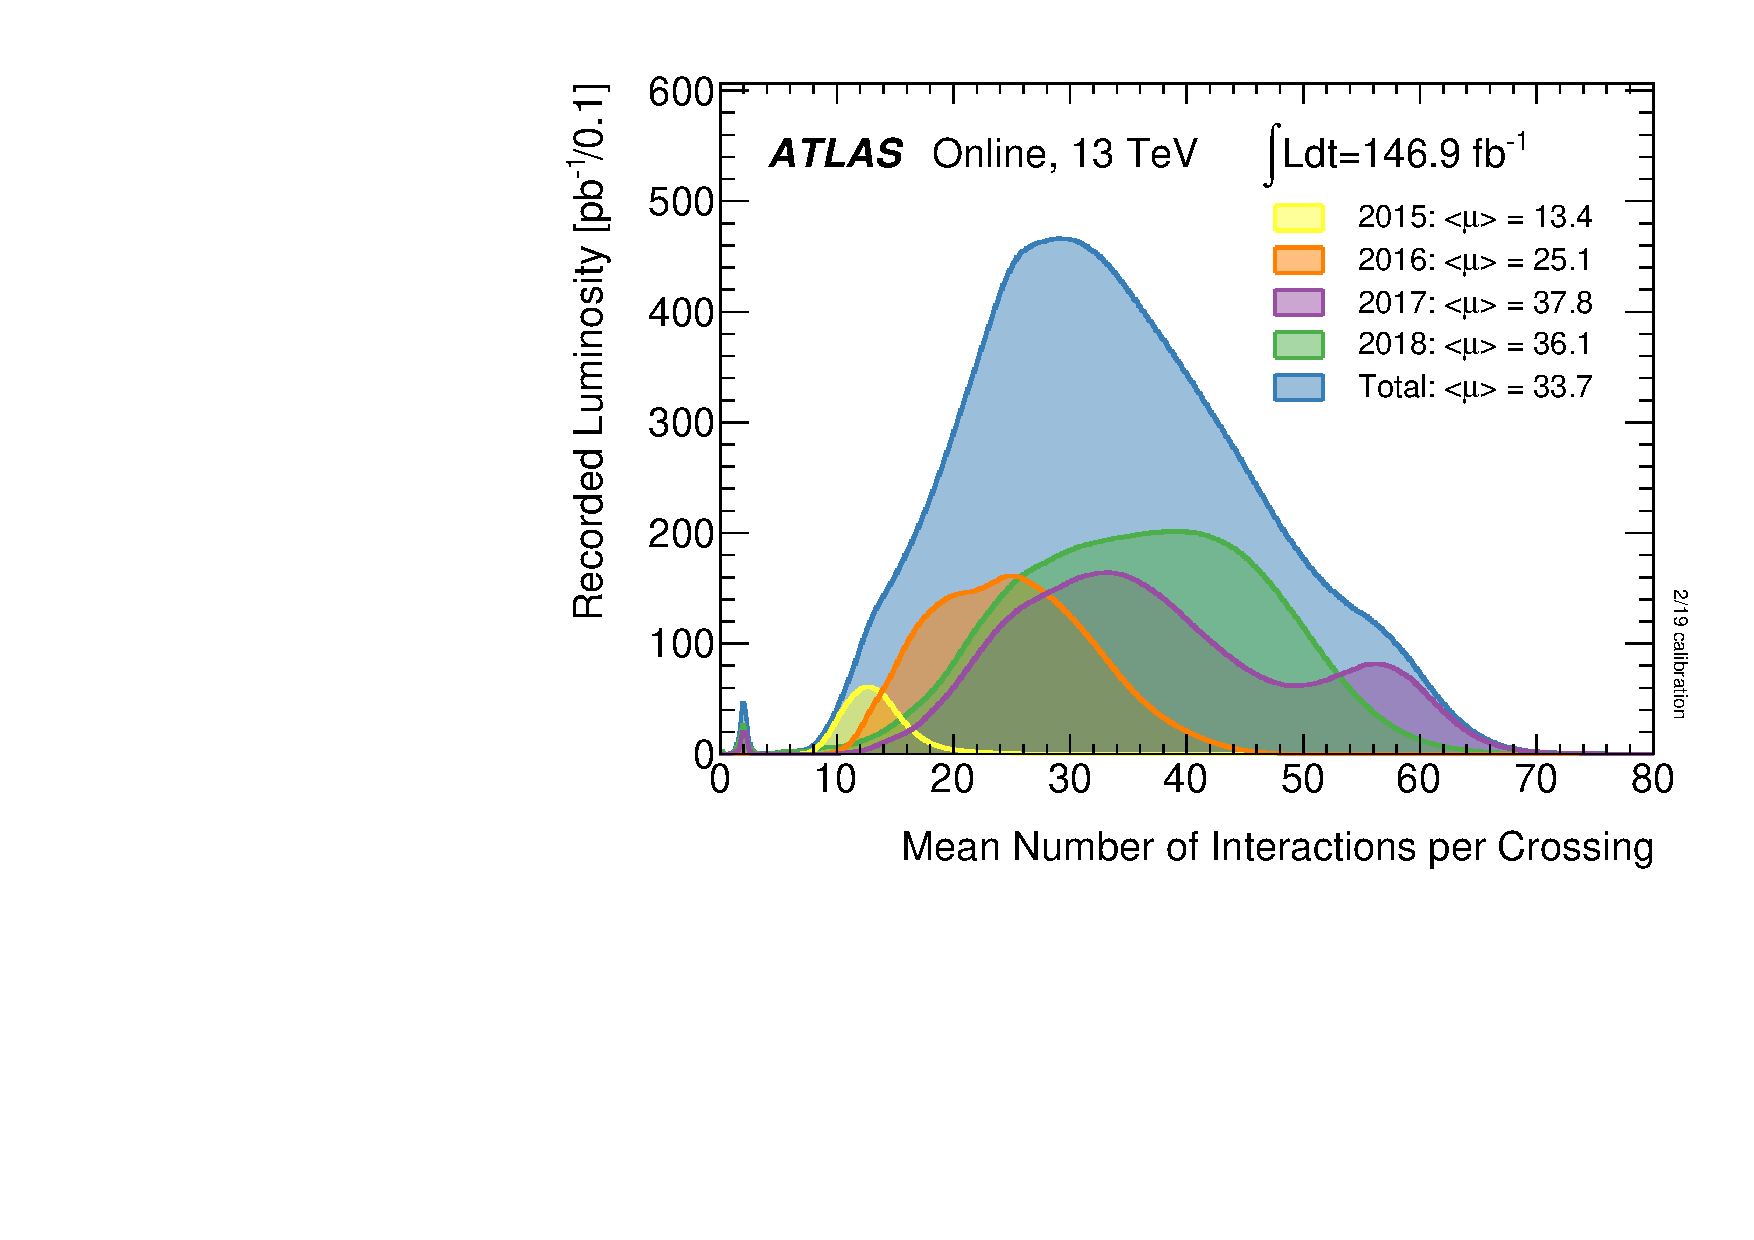
\includegraphics[width=0.9\linewidth]{figures/lhc/pileup.pdf}
    \caption{ Pileup for data taking periods 2015 - 2018 \cite{LuminosityPublicResultsRun2}.} 
    \label{fig:pileup} 
  \end{center} 
\end{figure}

The pile-up profile for past years can be seen in \Cref{fig:pileup}.  The width
of this distribution is due to a combination of Poissonian statistics, the
decrease in number of protons per bunch over the lifetime of a single run, and
optimization tweaks to the beam's profile during the LHC's operation.
Understanding and eliminating the unwanted contributions from these pile-up
events is crucial to reconstructing physics variables that describe the primary
interaction being observed.
